Din punctul de vedere al unui dezvoltator software am observat în timpul experienței faptul că pentru echipa efectivă de dezvoltare era destul de dificil de întretinut baza de date (mă refer chiar și la pornit/oprit, mai ales pentru juniori acest lucru putea pune probleme dacă baza de date se afla instalată pe o platforma UNIX). În cazul în care se dorea aplicarea unei strategii de point in time recovery pentru restabilirea bazei de date la o stare existentă la un moment dat, era nevoie de intervenția echipei de devOps, ceea ce se factură diferit la client, prin urmare trebuia convins în prealabil Product Owner-ul de necesitatea acelei intervenții si planificat totul.
\par
Astfel că, am observat necesitatea existenței unei aplicații care să ușureze operațiile asupra bazei de date, începând cu pornirea/oprirea/verificarea statusului până la întreaga operație de backup și point in time recovery(întoarcere la o stare existentă la un anumit moment dat). Aceasta aplicație trebuia să fie intuitivă, ușor de folosit chiar și pentru cineva care nu avea cunoștinte de devOps, nefiind necesar accesul efectiv pe mașina de UNIX unde se afla clusterul de baze de date. Este de la sine înteles că aplicația ar trebui să detecteze toate bazele de date din clusterul de pe mașina pe care este încărcată și ar trebui să permită operațiile prezentate mai sus pentru fiecare instanță în parte.
\par
Am propus o soluție pentru bazele de date PostgreSQL folosite pe platforme UNIX (la momentul de față). Pentru a prezenta soluția software am avut nevoie de un mediu UNIX pe care să ruleze un numar de instanțe PostgreSQL. Am ales o mașină CentOS, instanța EC2 oferită de Amazon. Sistemul de fișiere a fost organizat folosind LVM (logical volume manager) dupa cum urmeaza:
\begin{itemize}
\item am cerut 3 discuri de câte 50GiB, Amazon EBS;
\item am creat cate un physical volume din fiecare din cele 3 discuri;
\item am creat un volume group și le-am adăugat acestuia;
\item am creat 6 logical volumes, 3 seturi de cate 2 logical volumes; un logical volume de 20GiB pentru datele din db și un logical volume de 10GiB pentru stocarea fișierelor WAL.
\end{itemize}
Au mai ramas 60GiB nealocați, aceștia putând fi folosiți ulterior. Dacă se observă că un client are nevoie de mai mult spațiu i se pot extinde logical volumes folosind din spațiul nealocat, acesta fiind marele avantaj al LVM. Bazele de date nu vor fi întrerupte cât timp se face extinderea logical volumes.
\par
Am setat astfel sistemul de fișiere pentru 3 instanțe diferite de baze de date PostgreSQL denumite lv-pgdata-1, lv-pgdata-2 si lv-pgdata-3. În \textit{Figura 1} este prezentată diagrama sistemului de fișiere.
\begin{figure}[h]
	\centering
	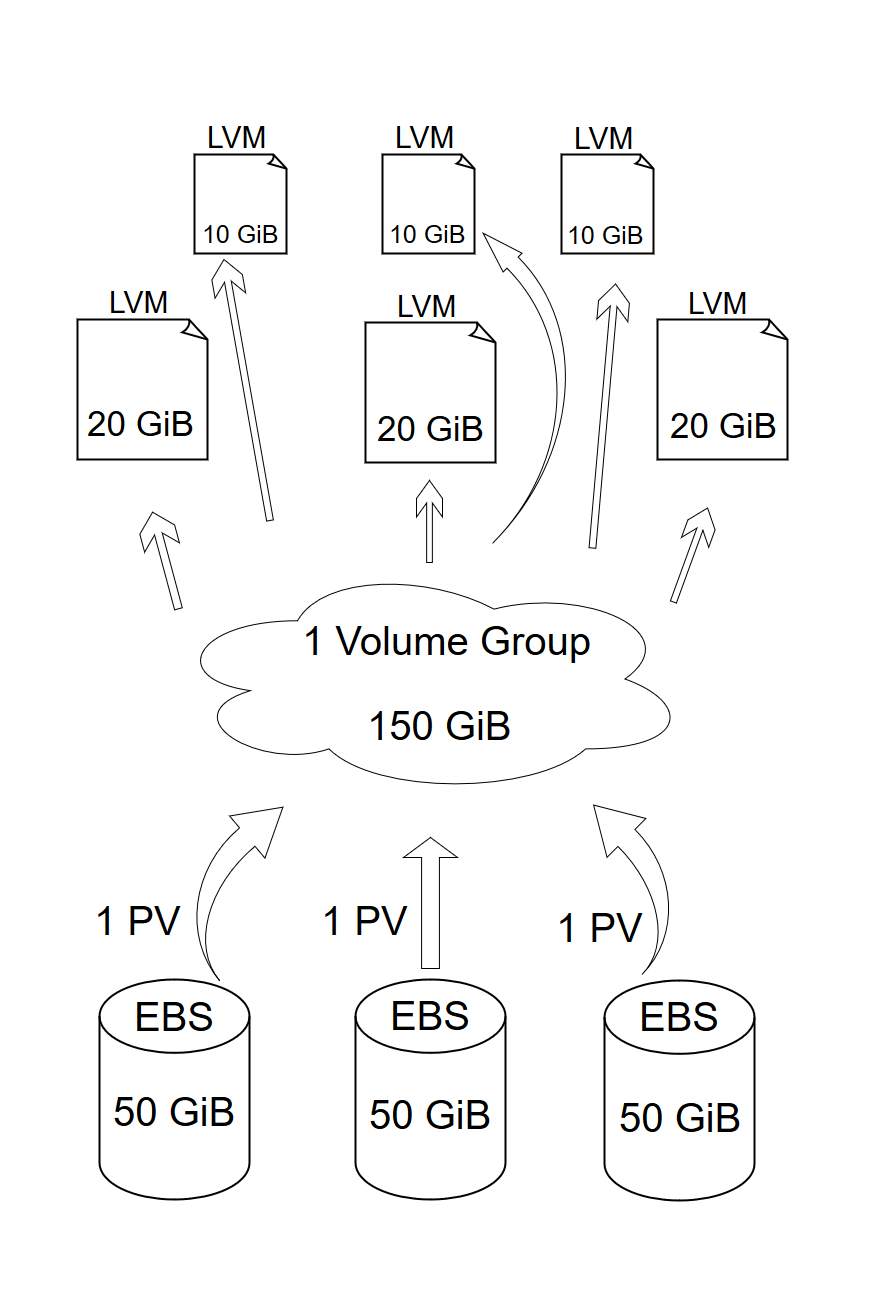
\includegraphics[scale=0.555]{LVM}
    \caption{Diagrama sistemului de fisiere}
    \label{fig:diagSistFiles}
\end{figure}